\documentclass{article}
\usepackage[utf8]{inputenc}
\usepackage{mathtools,mathptmx}

\usepackage{float}
\clearpage
\usepackage{natbib}
\usepackage{graphicx}
\usepackage{listings}
\usepackage{color} %red, green, blue, yellow, cyan, magenta, black, white
\definecolor{mygreen}{RGB}{28,172,0} % color values Red, Green, Blue
\definecolor{mylilas}{RGB}{170,55,241}


\usepackage[export]{adjustbox}
\usepackage{fourier} 
\usepackage{array}
\usepackage{makecell}

\renewcommand\theadalign{bc}
\renewcommand\theadfont{\bfseries}
\renewcommand\theadgape{\Gape[4pt]}
\renewcommand\cellgape{\Gape[4pt]}
% \renewcommand{\cellalign/theadalign}{vh}



\begin{document}

\begin{titlepage}
    \centering
    \vfill
    {\bfseries\Huge
        Visualising and Understanding Feature Maps in Instrument Classification \\
        \hphantom\\
        Project Specification
    }    
  	\vfill

    \vfill
    
\includegraphics[width=12cm]{queen-mary-logo.png} % also works with logo.pdf
    \vfill
    \vfill
    {\bfseries\Large
    
        Student Name: Chiao-Wei, Wang
      \\Student ID: 180595785
      \\Email address: c.wang@se18.qmul.ac.uk
      \\ \hphantom
      \\Date: \today
      \\Recipient: Dr. Gy\"orgy Fazekas
      \\MSc Sound and Music Computing
      \\Queen Mary University of London
      \\School of Electronic Engineering and Computer Science


    }    
    \vfill
    \vfill
\end{titlepage}


\pagestyle{plain}
\pagenumbering{arabic}
\section{Introduction}

Human has exceptional ability to recognise musical instrument in a piece of music or recording. However, a computer does not have the ability to hear. To solve this problem, several researches focus on algorithms and probability models; other focus on machine learning techniques. One of the most widely used algorithms in audio and music researches is Convolution Neural Network. Many researches achieve exceptional result with this architecture. However, although the mathematical behaviour was designed and can be understood easily, CNN has be seen as a black-box procedure. Only a few researches investigate how and where this network extract information from. This project will focus on a binary classification between acoustic guitar and electric guitar recordings with Convolution Neural Network. However, apart from accuracy, it will emphasis on the hidden information, the feature maps, in the CNN architecture.\\
Acoustic and electric guitar have the same way to produce sound, vibrating the strings. Because they are both string instruments so that they have similar harmonic structure given the same note or chord. However, an acoustic guitar uses both nylon strings and steel strings. On the other hand, an electric guitar uses steel strings only. Furthermore, electric guitar usually recorded with other effects such as, distortion, overdrive and flanger. Some of the effects commonly used are wave shapers indicating either harmonic structure are changed or added, which leads to very different sound characteristics. Starting with these two instruments allows one to investigate the differences between models without too many uncontrolled variables. Although this project will only focus on two instruments, it can be extended with larger datasets to work toward understanding this black-box process. 

\section{Aim and Objectives}
\subsection{Aim}
This project will aim to learn the capacity of the CNN as well as improve the knowledge in instrument classification.

\subsection{Objectives}
This project will fulfil the following objectives.
\begin{itemize}
\item To explore machine learning techniques in recent audio and music researches.
\item To investigate the audio feature for music and audio classification.
\item To compare the accuracy of models created using different sets of feature.
\item To analyse the feature maps from CNN with different input resolution and de-convolution technique.
\item To improve the knowledge of instrument classification with CNN.
\end{itemize}

\section{Methodology}
\subsection{Data gathering and feature extraction}
    The audio samples will consist acoustic guitar samples and electric guitar samples from RWC instrument dataset. {[\cite{goto2003rwc}]} The transient will be captured by CNN onset detection by Madmom. {[\cite{bock2016madmom}]} After the onset is found, each audio sample will be normalised to prevent the model predict the classes by its amplitude. The feature extractor will be based on Librosa' library. {[\citep{mcfee2015librosa}]} The audio feature will be used in this project is Mel-Spectrogram. It has been proved to have well representation of audio information. {[\cite{choi2016explaining} and \cite{choi2015auralisation}]}\\
    Each sample will consist one second duration of audio after onset point. To investigate more detailed transformation in CNN, there will be three sets of features. The FFT window size of these three sets will remain constant, 2048. However, the hopping size and number of mel bin will be changed. The purpose of these settings is reduce variables in CNN. In order to use the same model for all three feature sets, when the mel-bin is doubled, the number of time frame should be halved. In this case, only the input data will be changed but the filter size, pooling size, stride, and number of nodes will remain the same. Thus, this design can minimise the variation in CNN but be focus on input features and transformation in hidden layers.\\
    The first set of feature will have 128 frequency bins and 16 frames, which will have finest frequency resolution but lowest time resolution. The second set of feature will have half of number of frequency bins but the number of input frames will be doubled. The third set has finest frequency resolution but lowest time resolution. In this case, it will have 32 frequency bins and 64 time frames.
 
\subsection{Convolution Neural Network}
 
    The purpose of this research is not aiming at making the deepest network or highest accuracy. It will be focus on the hidden feature maps in the network. Thus, the model will be based on previous researches that have been proved successful in similar tasks. {[\cite{choi2016explaining} and \cite{choi2015auralisation}]}\\
    The proposed model will have 5 convolution layers and 2 fully-connected layer. The filter size will be 3 $\times$ 3 with pooling stride of 2 $times$ 2. The weight will be initialised with Xavier Initialisation.  {[\citep{glorot2010understanding}]} This initialisation method helps solve gradient vanishing problem. However, \cite{kumar2017weight} shows that Xavier Initialisation does not work well with the most popular activation function, ReLU. Thus, SeLU is selected for the project. {[\citep{klambauer2017self}]} SeLU has two strengths over ReLU. First, it is proved that SeLU works well with Xavier Initialisation. {[\citep{jiang2017effective}]} Secondly, this activation function contains the benefits of batch normalisation. Batch normalisation is a generally accepted method that helps the CNN to convergence. {[\citep{ioffe2015batch}} Furthermore, the model will also use dropout technique to prevent over-fitting. {[\citep{srivastava2014dropout}]} The dropout rate will remain the same for three models.\\
    The final output of the network will be passed into a Softmax function to model the probability that the samples belong to different classes. Cross-entropy cost function is selected as the output and prediction will not be in the same space. When training the network, it is very likely to get stuck in local minina. An inadequate learning rate will also makes the model difficult to converge. Thus, the model will be trained with stochastic batch gradient descent. It minimise the chance that a model is stuck in a local minima. Furthermore, Adam optimiser will be used. It not only has adaptive learning rate but also keeps the momentum. It is also widely used and has been proved very successful. {[\citep{kingma2014adam}}
   
\subsection{Accuracy and Feature Map Evaluation}
    In terms of evaluation method, there will be two main aspects. One of them focus on accuracy and the other one pay attention to the feature maps. The model will use training data to minimise the cross-entropy cost but the performance will be evaluate with testing data. Once the model is trained, the prediction can be calculated by passing the testing data into the model. The accuracy of the model can be evaluated by comparing prediction and the ground truth. The accuracy can be simply written as :
    \[
        \text{accuracy} = \frac{\text{number of correct prediction}}{\text{number of total prediction}}
    \]
    In statistical analysis of binary classification, F-measure can be also used as accuracy evaluation tool. F-measure consists two element: Precision(P) and Recall (R). Precision and Recall are given by:
    \[
        P = \frac{C}{C+F_P}
    \]
    \[
        R = \frac{C}{C+F_N}
    \]
    where:
    \begin{itemize}
        \item[P] is Precision
        \item[C] is the number of correct prediction
        \item[$F_P$] is number of false positive
        \item[$F_N$] is number of false negative
    \end{itemize}
    The F-score (F) is measured by:
    \[
        F = \frac{2PR}{P+R}
    \]
    
    A Receiver Operating Characteristic (ROC) curve is a graphical plot that shows the diagnostic ability of a binary classifier. True-positive rate (TPR) and false-positive rate (FPR) are known as sensitivity and fall-out and are given by:
    \[
        TPR = \frac{T_P}{T_P+F_N}
    \]
    \[
        FPR = \frac{F_P}{F_P+T_N}    
    \]
    where:
    \begin{itemize}
        \item[$T_P$] is number of true positive
        \item[$T_N$] is number of true negative
    \end{itemize}
    The ROC curve is created by plotting the TPR against the FPR with different threshold settings. The Area Under the ROC Curve (AUC) is widely used in machine learning researches. It provides an aggregate measure of performance across all possible classification thresholds by integrating from 0 to 1. \\
    These three evaluation tools will be used to examine the validity of the model. Furthermore, T-test and ANOVA test will be examined to investigate if the resolution affect the model accuracy. \\
    \cite{choi2015auralisation} and \cite{choi2016explaining} show the de-convolution method to visualise the feature maps. Other image researches use heat maps with a threshold to visualise the feature maps. {[\cite{chen2017masquer}; \cite{zeiler2014visualizing}]} This project will utilise these two method. The hidden information will be de-convolved back into original size. There will be several feature maps example demonstrated in this project and discuss the differences in different classes and feature sets. The feature maps will be evaluated by passing two different samples from each class. In this way, the differences in frequency (vertical) and time (horizontal) can be visualised and compared.
    \hss
    \begin{center}
    \hspace*{-.5cm} 
        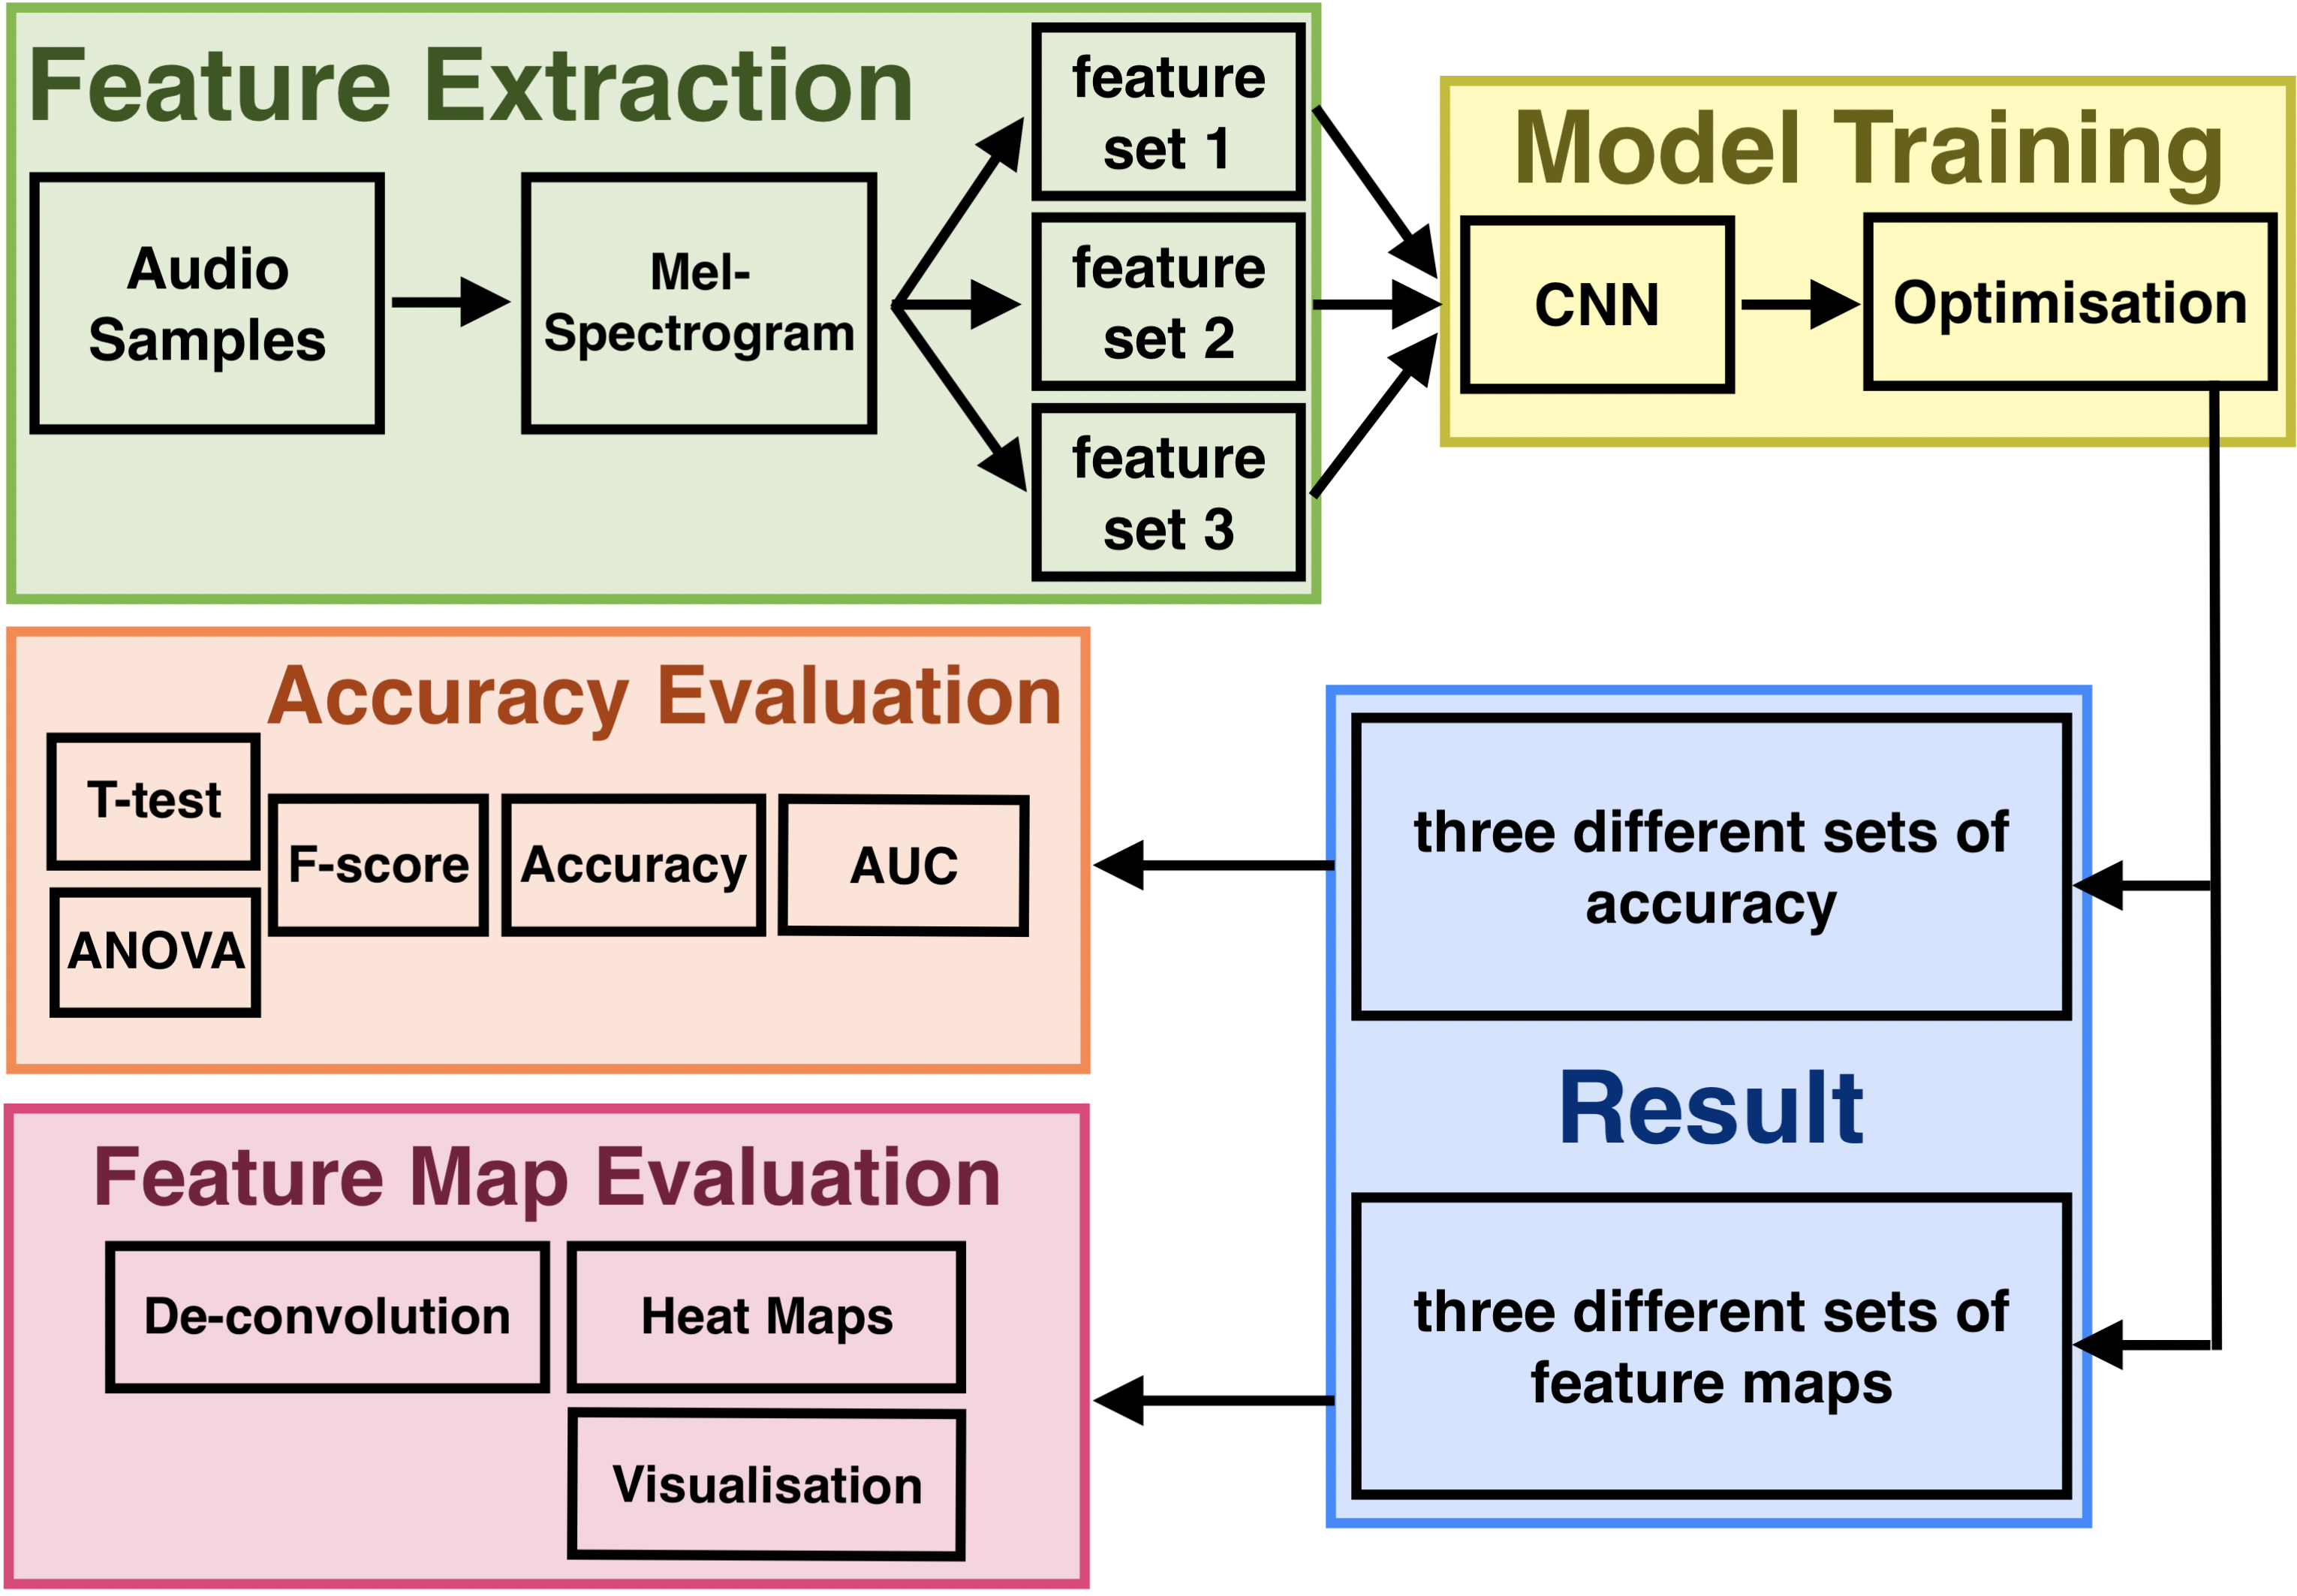
\includegraphics[width=\textwidth,height=\textheight,keepaspectratio]{3.png}
        \textbf{\large{Workflow of the project}}
    \end{center}
    
% \begin{figure}[H]
% \centering

% \caption{Workflow of the project.}
% \end{figure}
\clearpage
\section{Project Schedule}
To manage the project and make sure everything is covered in time. The use of a Gantt chart is an essential key. Tables below display the schedule containing starting time, duration, percentage of completion and the Gantt chart of the tasks for the project and the duration require. Also, there are several other actives and holidays added to make sure all works from the university are well concerned. There will be a regular meeting every two weeks with supervisors.\\

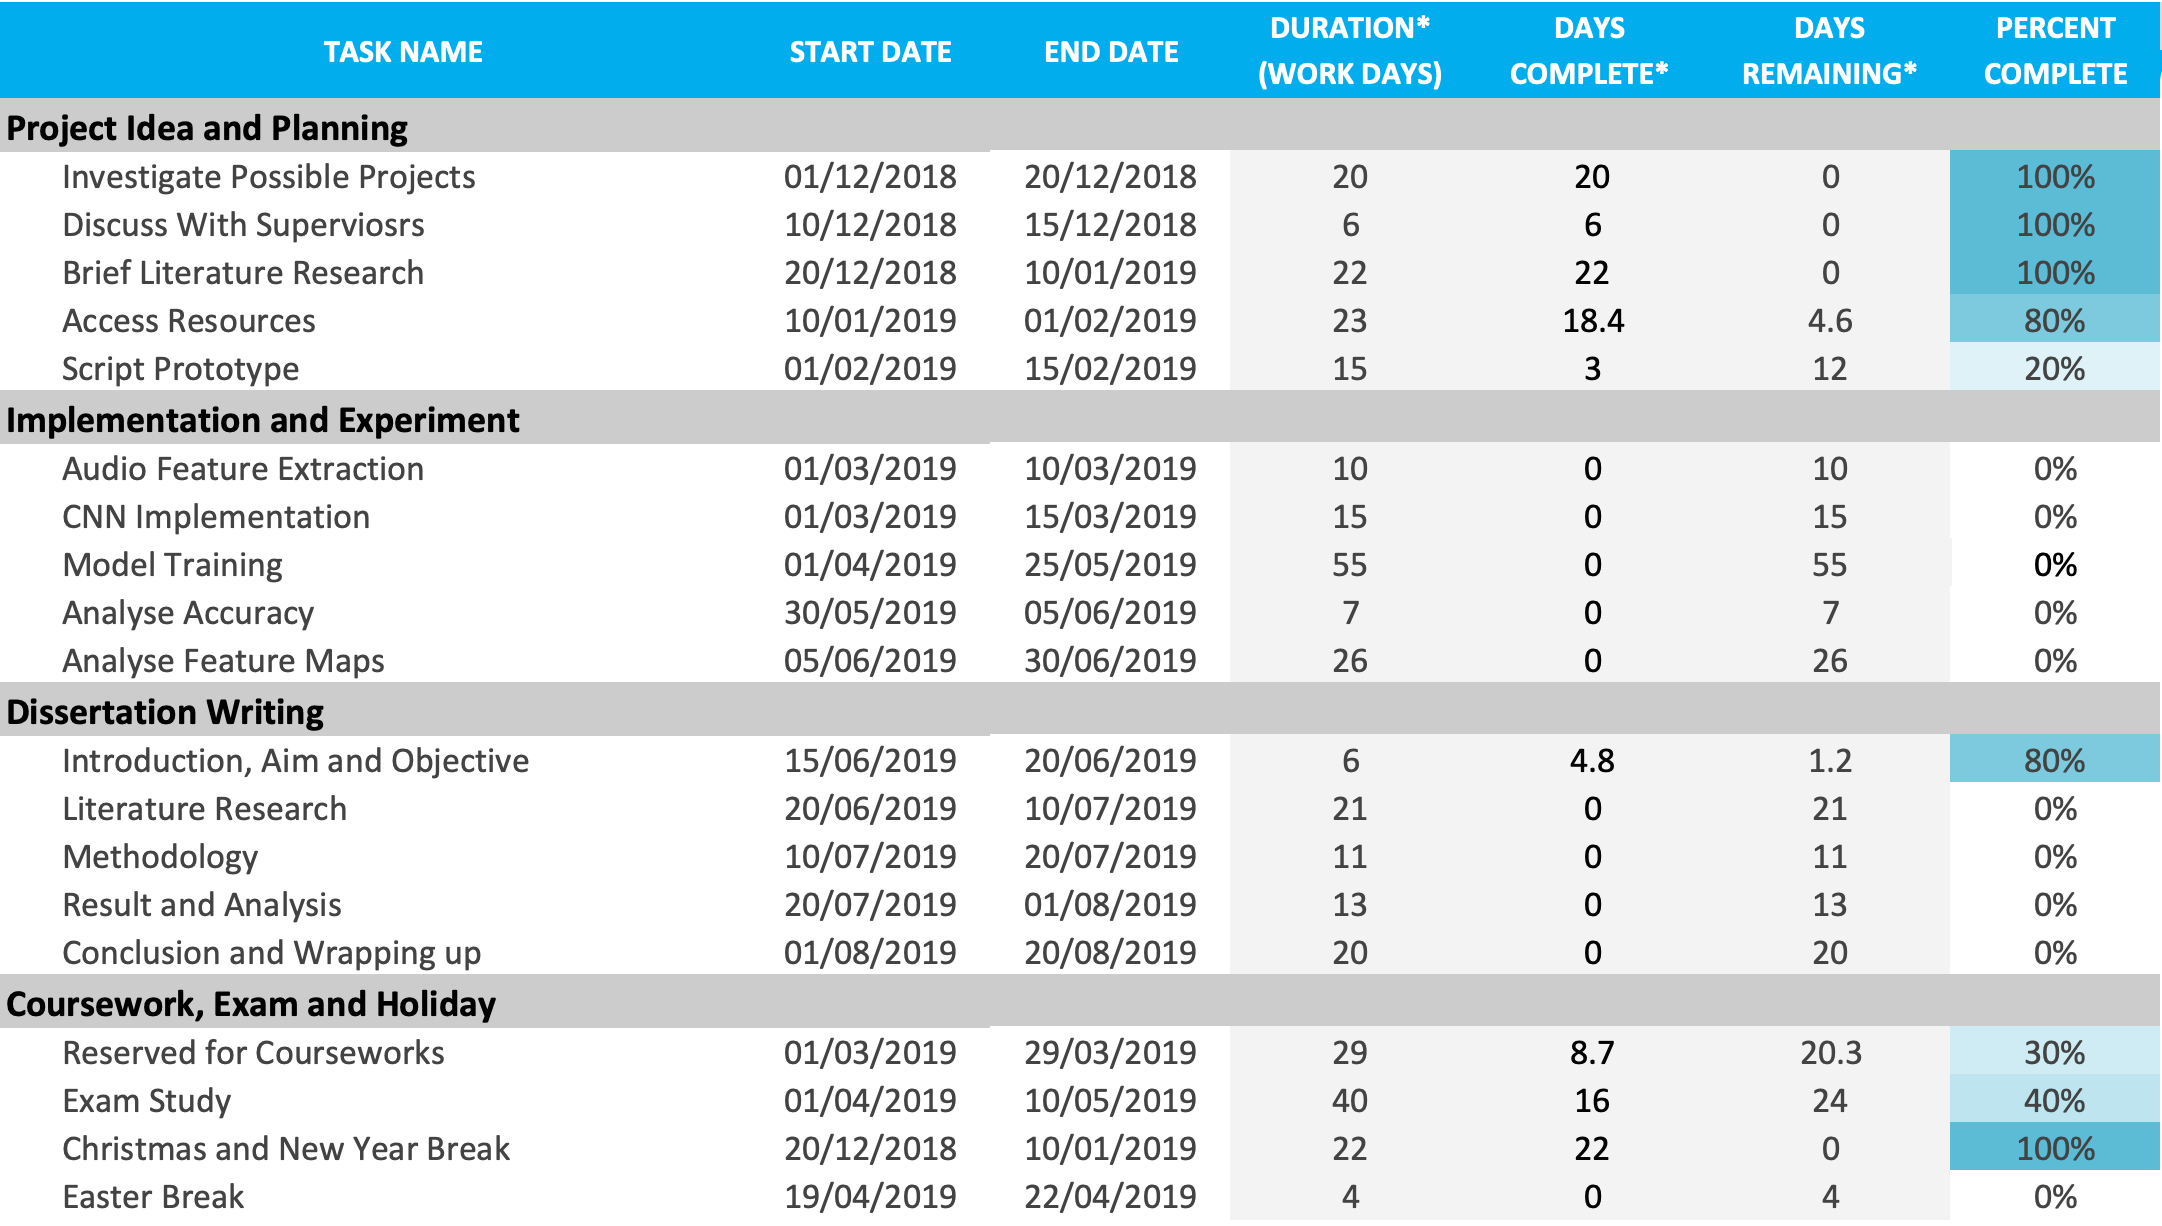
\includegraphics[width=12cm]{1.png}
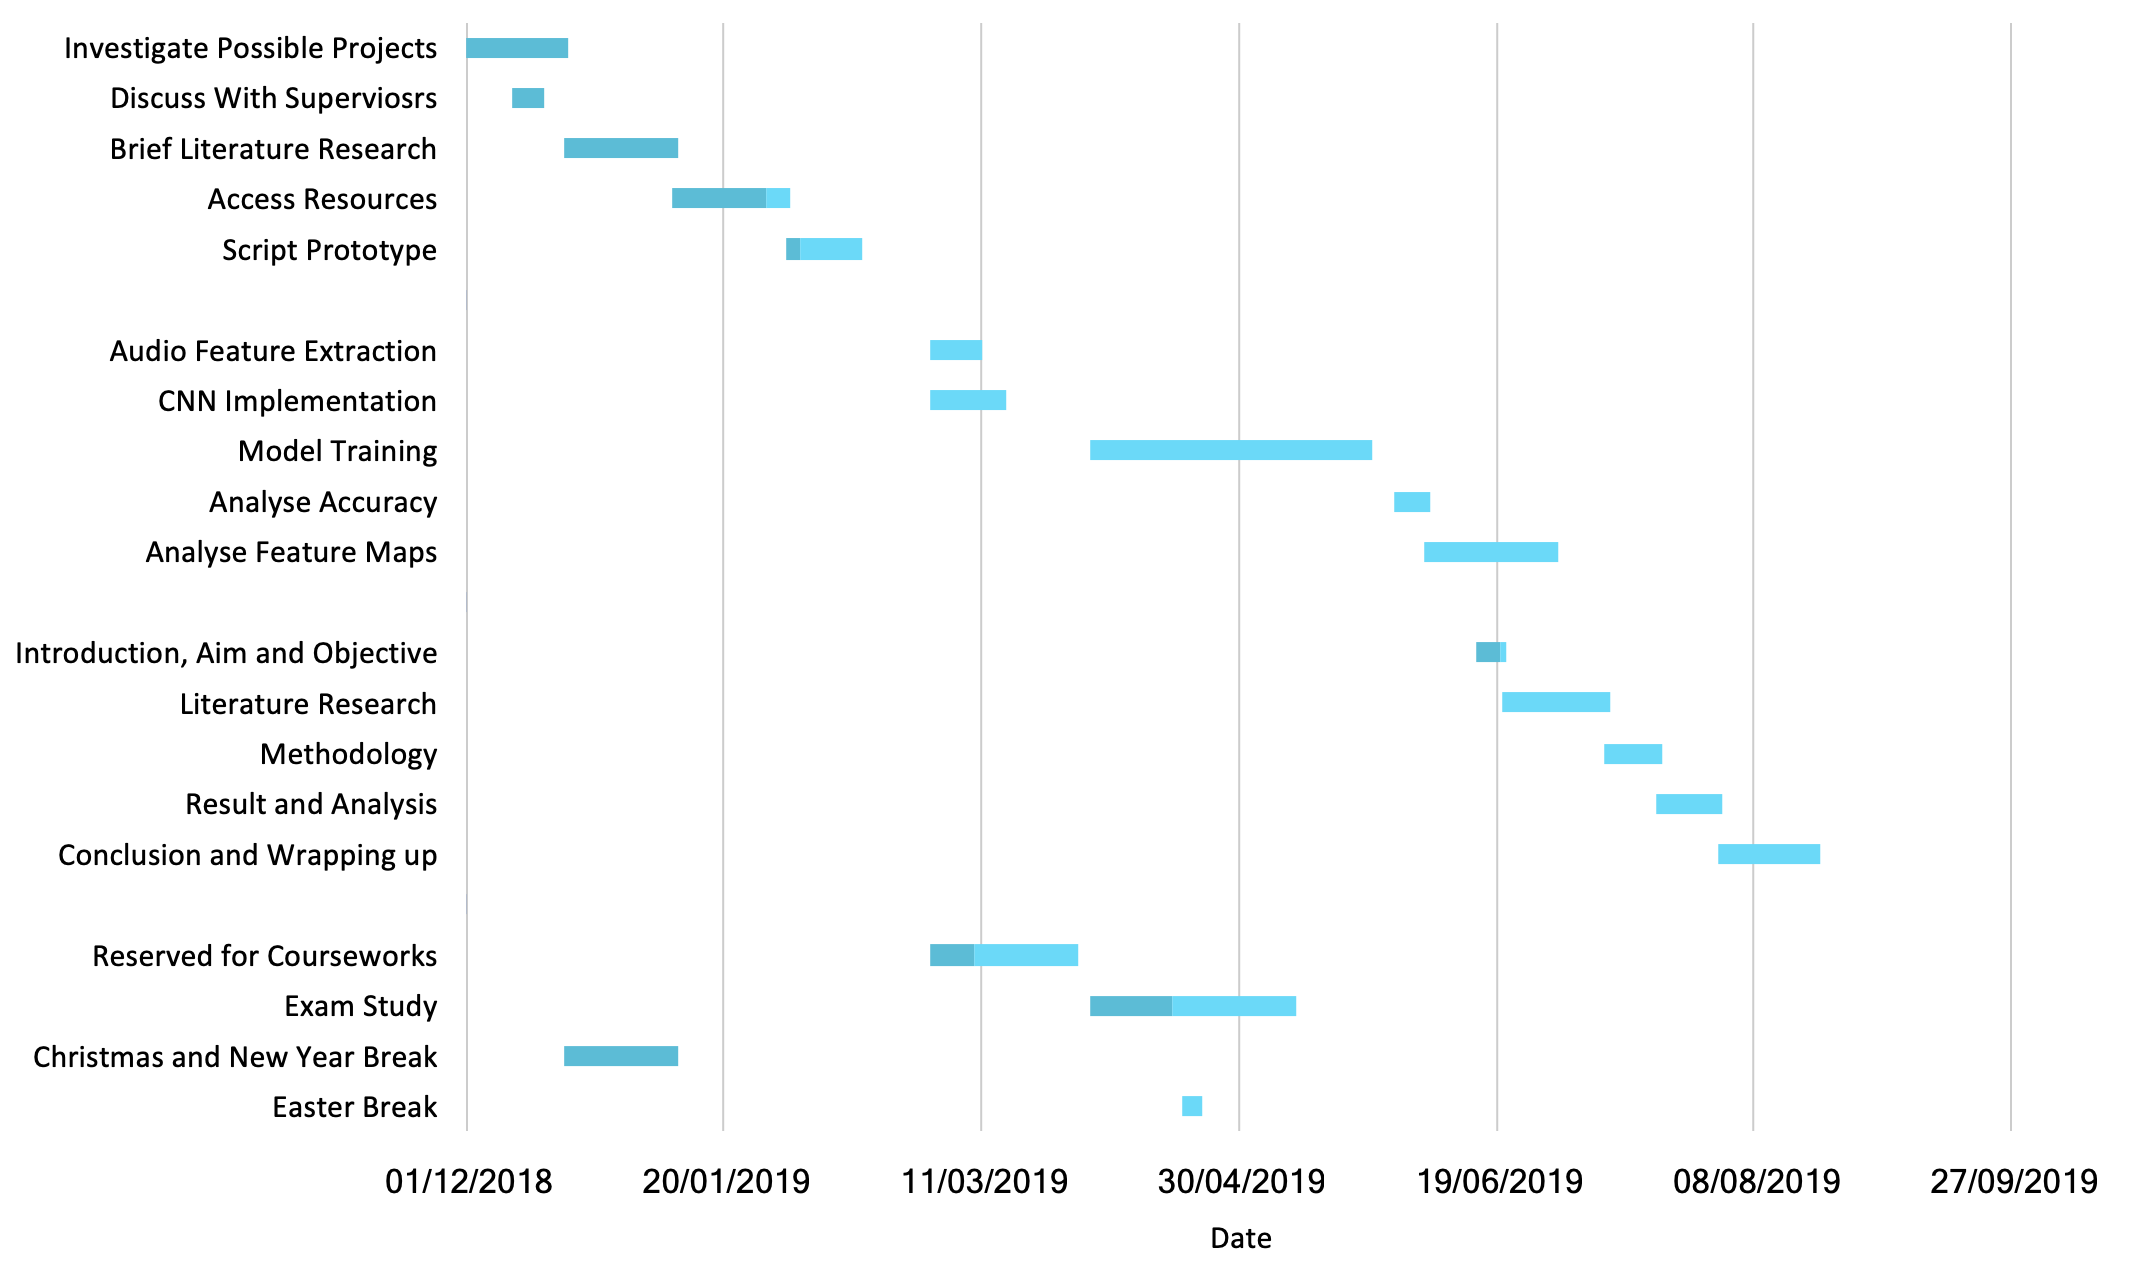
\includegraphics[width=12cm]{2.png}

\clearpage
\section{Risk Management}
Risk control is a part of managing the health and safety of a project. There are potential risks involved in the project but can be prevented. Table below shows the possible risks and the action to control risks. The risks were split into four categories, equipment and resource, technical, personal and management.
\subsection{Equipment and Resource}

\begin{table} [H]
\begin{adjustbox}{width=1\textwidth}
\begin{tabular}{|c|c|c|c|}  \hline
Risk Description&Likelihood&Impact&Mitigation Strategy \\ \hline \hline
\mekecell{Inappropriate audio samples} & Low & High & \makecell{Access other dataset} \\ \hline
Slow hardware & Low & Moderate & \makecell{AWS, GCP} \\ \hline
\makecell{Not enough data} & High & Moderate & \makecell{Apple Loops,\\ Multitrack Testbed} \\ \hline
\makecell{Crowded server} & Moderate & Low/Moderate & \makecell{AWS, \\time management}\\ \hline
\end{tabular}
\end{adjustbox}
\end{table}

\subsection{Technical}

\begin{table} [H]
\begin{adjustbox}{width=1\textwidth}
\begin{tabular}{|c|c|c|c|}  \hline
Risk Description&Likelihood&Impact&Mitigation Strategy \\ \hline \hline
\mekecell{Low quality model} & Moderate & Moderate & \makecell{Investigate other works} \\ \hline
Not convergence & Low & High & \makecell{Hyperparameter Setting} \\ \hline
\makecell{Audio feature\\not discriminating} & Moderate & Moderate & \makecell{Access other algorithm} \\ \hline
\makecell{Difficulties in \\evaluating feature map} & High & High & \makecell{Seek for papers,\\ talk to c4dm specialist}\\ \hline
\end{tabular}
\end{adjustbox}
\end{table}

\subsection{Personal}

\begin{table} [H]
\begin{adjustbox}{width=1\textwidth}
\begin{tabular}{|c|c|c|c|}  \hline
Risk Description&Likelihood&Impact&Mitigation Strategy \\ \hline \hline
\mekecell{Coding ability} & Low & High & \makecell{Start with prototypes,\\ Github} \\ \hline
Writing ability & High & Moderate & \makecell{Time management,\\ seek for academic help} \\ \hline
\makecell{Eye abusing} & Moderate & Moderate & \makecell{Regular rest} \\ \hline
\makecell{Laziness} & Low & Moderate & \makecell{Follow time schedule,\\ regular meetings}\\ \hline
\end{tabular}
\end{adjustbox}
\end{table}

\subsection{Management}

\begin{table} [H]
\begin{adjustbox}{width=1\textwidth}
\begin{tabular}{|c|c|c|c|}  \hline
Risk Description&Likelihood&Impact&Mitigation Strategy \\ \hline \hline
\mekecell{Time} & High & High & \makecell{Gantt Chart} \\ \hline
Scope & Low & Low & \makecell{Regular meetings} \\ \hline
\makecell{Cost} & Low & Low & \makecell{Ask IT for \\resources} \\ \hline
\makecell{Writing paper} & Low & Moderate & \makecell{Follow time schedule,\\ start earlier}\\ \hline
\end{tabular}
\end{adjustbox}
\end{table}

\section{Ethics Review}
The data will be used in this project are open-sourced dataset. All third-party Python libraries mentioned are open-sourced as well. The dataset is collected by c4dm and both the supervisor and IT centre approved the use of the dataset in this project. Also, the collected data will not be used in commercial or any re-mix and publishing.
\clearpage
\bibliographystyle{agsm}
\bibliography{references}

\end{document}








